%%%%%%%%%%%%%%%%%%%%%%%%%%%%%%%%%%%%%%%%%
% Beamer Presentation
% LaTeX Template
% Version 1.0 (10/11/12)
%
% This template has been downloaded from:
% http://www.LaTeXTemplates.com
%
% License:
% CC BY-NC-SA 3.0 (http://creativecommons.org/licenses/by-nc-sa/3.0/)
%
%%%%%%%%%%%%%%%%%%%%%%%%%%%%%%%%%%%%%%%%%

%----------------------------------------------------------------------------------------
%	PACKAGES AND THEMES
%----------------------------------------------------------------------------------------

\documentclass[xcolor=table]{beamer}

\mode<presentation> {

% The Beamer class comes with a number of default slide themes
% which change the colors and layouts of slides. Below this is a list
% of all the themes, uncomment each in turn to see what they look like.

\usetheme{default}
%\usetheme{AnnArbor}
%\usetheme{Antibes}
%\usetheme{Bergen}
%\usetheme{Berkeley}
%\usetheme{Berlin}
%\usetheme{Boadilla}
%\usetheme{CambridgeUS}
%\usetheme{Copenhagen}
%\usetheme{Darmstadt}
%\usetheme{Dresden}
%\usetheme{Frankfurt}
%\usetheme{Goettingen}
%\usetheme{Hannover}
%\usetheme{Ilmenau}
%\usetheme{JuanLesPins}
%\usetheme{Luebeck}
%\usetheme{Madrid}
%\usetheme{Malmoe}
%\usetheme{Marburg}
%\usetheme{Montpellier}
%\usetheme{PaloAlto}
%\usetheme{Pittsburgh}
%\usetheme{Rochester}
%\usetheme{Singapore}
%\usetheme{Szeged}
%\usetheme{Warsaw}

% As well as themes, the Beamer class has a number of color themes
% for any slide theme. Uncomment each of these in turn to see how it
% changes the colors of your current slide theme.

%\usecolortheme{albatross}
%\usecolortheme{beaver}
%\usecolortheme{beetle}
%\usecolortheme{crane}
%\usecolortheme{dolphin}
%\usecolortheme{dove}
%\usecolortheme{fly}
%\usecolortheme{lily}
%\usecolortheme{orchid}
%\usecolortheme{rose}
%\usecolortheme{seagull}
%\usecolortheme{seahorse}
%\usecolortheme{whale}
%\usecolortheme{wolverine}
%\setbeamertemplate{footline} % To remove the footer line in all slides uncomment this line
\setbeamertemplate{footline}[page number] % To replace the footer line in all slides with a simple slide count uncomment this line

\setbeamertemplate{navigation symbols}{} % To remove the navigation symbols from the bottom of all slides uncomment this line 
}
\usepackage{amsmath} 
\usepackage{graphicx} % Allows including images
\usepackage{booktabs} % Allows the use of \toprule, \midrule and \bottomrule in tables
\usepackage[table]{xcolor}
\usepackage{pgfplots}
\usepackage{tcolorbox}
\pgfplotsset{compat=1.15}
\usepackage{mathrsfs}
\usetikzlibrary{arrows}
\usetikzlibrary{patterns}


\usepackage{tikz}
\usepackage{pstricks-add}
\usetikzlibrary{arrows,shapes,positioning,shadows,trees}


\usepackage{tcolorbox}
\usepackage{wrapfig}


\usepackage{hyperref}
\hypersetup{
    colorlinks,
    citecolor=black,
    filecolor=black,
    linkcolor=black,
    urlcolor=black
}
\newcommand{\notimplies}{%
    \mathrel{{\ooalign{\hidewidth$\not\phantom{=}$\hidewidth\cr$\implies$}}}}


\DeclareMathAlphabet\mathzapf{T1}{pzc}{mb}{it}
\usepackage{amsmath,wasysym}
\usepackage{latexsym}

\usepackage{amssymb}
\usepackage{mathrsfs}
\usepackage{bm}
\usepackage{wrapfig}
\usepackage{fancybox}
\bibliographystyle{amsplain}
\usepackage{systeme}
\usepackage{pdfpages}


\usepackage{yfonts}
\usepackage[french]{babel}



\usepackage[T2A]{fontenc}




%\usepackage[style=ieee]{biblatex} %Use if necessary for citation
%\addbibresource{biblatex-examples.bib}
%----------------------------------------------------------------------------------------
%	TITLE PAGE
%----------------------------------------------------------------------------------------

\title[Physique]{Introduction à la Mécanique II} % The short title appears at the bottom of every slide, the full title is only on the title page

\author{Team Physique} % Your name
\institute[S4S] % Your institution as it will appear on the bottom of every slide, may be shorthand to save space
{
initiative S4S\\ % Your institution for the title page
\medskip
}
\date{\today} % Date, can be changed to a custom date

\begin{document}
\begin{frame}
\titlepage % Print the title page as the first slide
\end{frame}


\begin{frame}{Coordonnées polaires I}
\begin{center}
    
\definecolor{uuuuuu}{rgb}{0.26666666666666666,0.26666666666666666,0.26666666666666666}
\begin{tikzpicture}[line cap=round,line join=round,>=triangle 45,x=2.0833333333333335cm,y=2.0833333333333335cm]
\begin{axis}[
x=2.0833333333333335cm,y=2.0833333333333335cm,
axis lines=middle,
ymajorgrids=true,
xmajorgrids=true,
xmin=-1.2,
xmax=1.2,
ymin=-1.2,
ymax=1.2,
xtick={-1.0,-0.5,...,1.2000000000000002},
ytick={-1.0,-0.5,...,1.2000000000000002},]
\clip(-1.2,-1.2) rectangle (1.2,1.2);
\draw[line width=4.pt] (-1.5792450881463642,1.523861171936301) -- (-0.922637072324789,1.523861171936301);
\begin{scriptsize}
\draw [fill=black] (-1.1403349603009507,1.523861171936301) circle (2.5pt);
\draw[color=black] (-1.0670908358055355,1.601012613795336) node {$alpha = 4.2$};
\draw [fill=uuuuuu] (-0.4902608213406994,-0.8715757724135882) circle (2.0pt);
\draw[color=uuuuuu] (0.07,0.07) node {$O$};
\draw[color=uuuuuu] (-0.4662945013287942,-0.75) node {$B$};
\draw [fill=uuuuuu] (-0.5748239465332692,-0.8182771110644103) circle (2.0pt);
\draw [fill=uuuuuu] (-0.32328956686350335,0.9463000876874145) circle (2.0pt);
\draw [fill=uuuuuu] (0.6967067093471654,0.7173560908995228) circle (2.0pt);
\draw [fill=uuuuuu] (0.8253356149096783,0.5646424733950354) circle (2.0pt);
\draw [fill=uuuuuu] (1.,0.) circle (2.0pt);
\draw [fill=uuuuuu] (0.9210609940028851,0.3894183423086505) circle (2.0pt);
\draw [fill=uuuuuu] (0.8775825618903728,0.479425538604203) circle (2.0pt);
\draw [fill=uuuuuu] (0.8253356149096783,0.5646424733950354) circle (2.0pt);
\draw [fill=uuuuuu] (0.7648421872844885,0.644217687237691) circle (2.0pt);
\draw [fill=uuuuuu] (0.6967067093471654,0.7173560908995228) circle (2.0pt);
\draw [fill=uuuuuu] (0.6216099682706644,0.7833269096274834) circle (2.0pt);
\draw [fill=uuuuuu] (0.5403023058681398,0.8414709848078965) circle (2.0pt);
\draw [fill=uuuuuu] (0.4535961214255773,0.8912073600614354) circle (2.0pt);
\draw [fill=uuuuuu] (0.3623577544766736,0.9320390859672263) circle (2.0pt);
\draw [fill=uuuuuu] (0.26749882862458735,0.963558185417193) circle (2.0pt);
\draw [fill=uuuuuu] (0.16996714290024104,0.9854497299884601) circle (2.0pt);
\draw [fill=uuuuuu] (-0.2272020946930871,0.9738476308781951) circle (2.0pt);
\draw [fill=uuuuuu] (-0.32328956686350335,0.9463000876874145) circle (2.0pt);
\draw [fill=uuuuuu] (-0.4161468365471424,0.9092974268256817) circle (2.0pt);
\draw [fill=uuuuuu] (-0.8568887533689473,0.5155013718214642) circle (2.0pt);
\draw [fill=uuuuuu] (-0.9040721420170612,0.4273798802338298) circle (2.0pt);
\draw [fill=uuuuuu] (-0.9422223406686581,0.3349881501559051) circle (2.0pt);
\draw [fill=uuuuuu] (-0.9040721420170612,0.4273798802338298) circle (2.0pt);
\draw [fill=uuuuuu] (-0.8568887533689473,0.5155013718214642) circle (2.0pt);
\draw [fill=uuuuuu] (-0.8011436155469337,0.5984721441039564) circle (2.0pt);
\draw [fill=uuuuuu] (-0.7373937155412454,0.675463180551151) circle (2.0pt);
\draw [fill=uuuuuu] (-0.5048461045998576,0.8632093666488737) circle (2.0pt);
\draw [fill=uuuuuu] (-0.32328956686350335,0.9463000876874145) circle (2.0pt);
\draw [fill=uuuuuu] (-0.2272020946930871,0.9738476308781951) circle (2.0pt);
\draw [fill=uuuuuu] (0.0707372016677029,0.9974949866040544) circle (2.0pt);
\draw [fill=uuuuuu] (0.3623577544766736,0.9320390859672263) circle (2.0pt);
\draw [fill=uuuuuu] (0.4535961214255773,0.8912073600614354) circle (2.0pt);
\draw [fill=uuuuuu] (0.5403023058681398,0.8414709848078965) circle (2.0pt);
\draw [fill=uuuuuu] (0.4535961214255773,0.8912073600614354) circle (2.0pt);
\draw [fill=uuuuuu] (0.16996714290024104,0.9854497299884601) circle (2.0pt);
\draw [fill=uuuuuu] (-0.12884449429552464,0.9916648104524686) circle (2.0pt);
\draw [fill=uuuuuu] (-0.2272020946930871,0.9738476308781951) circle (2.0pt);
\draw [fill=uuuuuu] (-0.32328956686350335,0.9463000876874145) circle (2.0pt);
\draw [fill=uuuuuu] (-0.4161468365471424,0.9092974268256817) circle (2.0pt);
\draw [fill=uuuuuu] (-0.5048461045998576,0.8632093666488737) circle (2.0pt);
\draw [fill=uuuuuu] (-0.5885011172553458,0.8084964038195901) circle (2.0pt);
\draw [fill=uuuuuu] (-0.7373937155412454,0.675463180551151) circle (2.0pt);
\draw [fill=uuuuuu] (-0.8568887533689473,0.5155013718214642) circle (2.0pt);
\draw [fill=uuuuuu] (-0.9991351502732795,0.04158066243329049) circle (2.0pt);
\draw [fill=uuuuuu] (-0.9982947757947531,-0.058374143427580086) circle (2.0pt);
\draw [fill=uuuuuu] (-0.9874797699088649,-0.1577456941432482) circle (2.0pt);
\draw [fill=uuuuuu] (-0.9991351502732795,0.04158066243329049) circle (2.0pt);
\draw [fill=uuuuuu] (-0.9899924966004454,0.1411200080598672) circle (2.0pt);
\draw [fill=uuuuuu] (-0.9422223406686581,0.3349881501559051) circle (2.0pt);
\draw [fill=uuuuuu] (-0.9040721420170612,0.4273798802338298) circle (2.0pt);
\draw [fill=uuuuuu] (-0.8011436155469337,0.5984721441039564) circle (2.0pt);
\draw [fill=uuuuuu] (-0.8568887533689473,0.5155013718214642) circle (2.0pt);
\draw [fill=uuuuuu] (-0.9040721420170612,0.4273798802338298) circle (2.0pt);
\draw [fill=uuuuuu] (-0.9709581651495905,0.23924932921398243) circle (2.0pt);
\draw [fill=uuuuuu] (-0.9991351502732795,0.04158066243329049) circle (2.0pt);
\draw [fill=uuuuuu] (-0.9982947757947531,-0.058374143427580086) circle (2.0pt);
\draw [fill=uuuuuu] (-0.9874797699088649,-0.1577456941432482) circle (2.0pt);
\draw [fill=uuuuuu] (-0.9667981925794611,-0.2555411020268312) circle (2.0pt);
\draw [fill=uuuuuu] (-0.896758416334147,-0.44252044329485246) circle (2.0pt);
\draw [fill=uuuuuu] (-0.848100031710408,-0.5298361409084934) circle (2.0pt);
\draw [fill=uuuuuu] (-0.7909677119144168,-0.6118578909427189) circle (2.0pt);
\draw [fill=uuuuuu] (-0.7259323042001402,-0.6877661591839738) circle (2.0pt);
\draw [fill=uuuuuu] (-0.6536436208636119,-0.7568024953079282) circle (2.0pt);
\draw [fill=uuuuuu] (-0.5748239465332692,-0.8182771110644103) circle (2.0pt);
\draw [fill=uuuuuu] (0.5403023058681398,0.8414709848078965) circle (2.0pt);
\draw [fill=uuuuuu] (0.955336489125606,0.29552020666133955) circle (2.0pt);
\draw [fill=uuuuuu] (1.,0.) circle (2.0pt);
\draw [fill=uuuuuu] (0.9950041652780258,0.09983341664682815) circle (2.0pt);
\draw [fill=uuuuuu] (0.9800665778412416,0.19866933079506122) circle (2.0pt);
\draw [fill=uuuuuu] (0.955336489125606,0.29552020666133955) circle (2.0pt);
\draw [fill=uuuuuu] (0.16996714290024104,0.9854497299884601) circle (2.0pt);
\draw [fill=uuuuuu] (-0.7373937155412454,0.675463180551151) circle (2.0pt);
\draw [fill=uuuuuu] (-0.9709581651495905,0.23924932921398243) circle (2.0pt);
\draw [fill=uuuuuu] (-0.9899924966004454,0.1411200080598672) circle (2.0pt);
\draw [fill=uuuuuu] (-0.9991351502732795,0.04158066243329049) circle (2.0pt);
\draw [fill=uuuuuu] (-0.9982947757947531,-0.058374143427580086) circle (2.0pt);
\draw [fill=uuuuuu] (-0.9874797699088649,-0.1577456941432482) circle (2.0pt);
\draw [fill=uuuuuu] (-0.9667981925794611,-0.2555411020268312) circle (2.0pt);
\draw [fill=uuuuuu] (-0.9364566872907963,-0.35078322768961984) circle (2.0pt);
\draw [fill=uuuuuu] (-0.896758416334147,-0.44252044329485246) circle (2.0pt);
\draw [fill=uuuuuu] (-0.848100031710408,-0.5298361409084934) circle (2.0pt);
\draw [fill=uuuuuu] (-0.7909677119144168,-0.6118578909427189) circle (2.0pt);
\draw [fill=uuuuuu] (-0.7259323042001402,-0.6877661591839738) circle (2.0pt);
\draw [fill=uuuuuu] (-0.6536436208636119,-0.7568024953079282) circle (2.0pt);
\draw [fill=uuuuuu] (-0.5748239465332692,-0.8182771110644103) circle (2.0pt);
\draw [fill=uuuuuu] (-0.4902608213406994,-0.8715757724135882) circle (2.0pt);
\end{scriptsize}
\end{axis}
\end{tikzpicture}
\end{center}
    
\end{frame}

\begin{frame}{Coordonnées polaires II}
\centering
    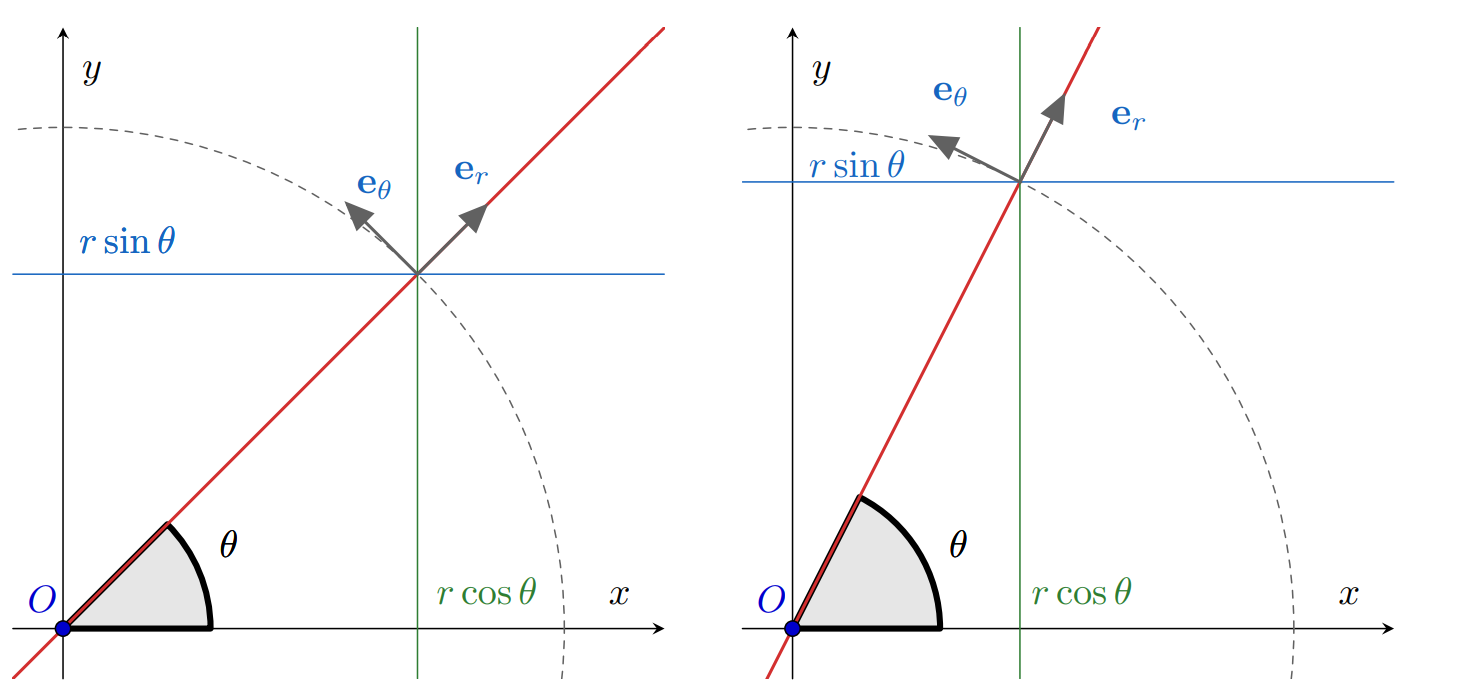
\includegraphics[scale = 0.6]{Images/Polaire}
\end{frame}


%\begin{frame}{Coordonnées polaires III}
%  Les relations liant les coordonnées cartésiennes aux coordonnées polaires sont les suivantes :
%\begin{equation}    
%\begin{cases} x = %r\cos{\theta} \\
%y = r\sin{\theta} 
%\end{cases}
%\end{equation}
%\end{frame}

\begin{frame}{Coordonnées cylindriques}
    \centering
    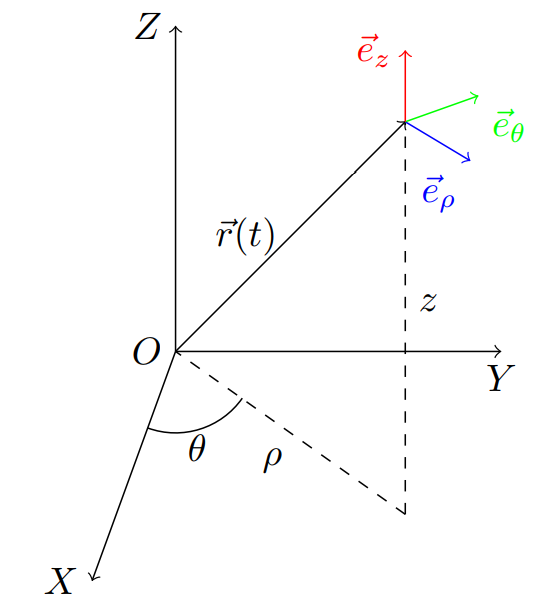
\includegraphics[scale = 0.9]{Images/Cylindrique}
\end{frame}

\begin{frame}{Coordonnées sphériques}
    \centering
    \includegraphics[scale = 0.9]{Images/sphérique}
\end{frame}

\begin{frame}{Oscillateur harmonique I}
   "Ce modèle mathématique décrit l'évolution de n'importe quel système physique au voisinage d'une position d'équilibre stable, ce qui en fait un outil transversal utilisé dans de nombreux domaines : mécanique, électricité et électronique, optique"
\end{frame}



\begin{frame}{Oscillateur harmonique II : Exemple}
\centering
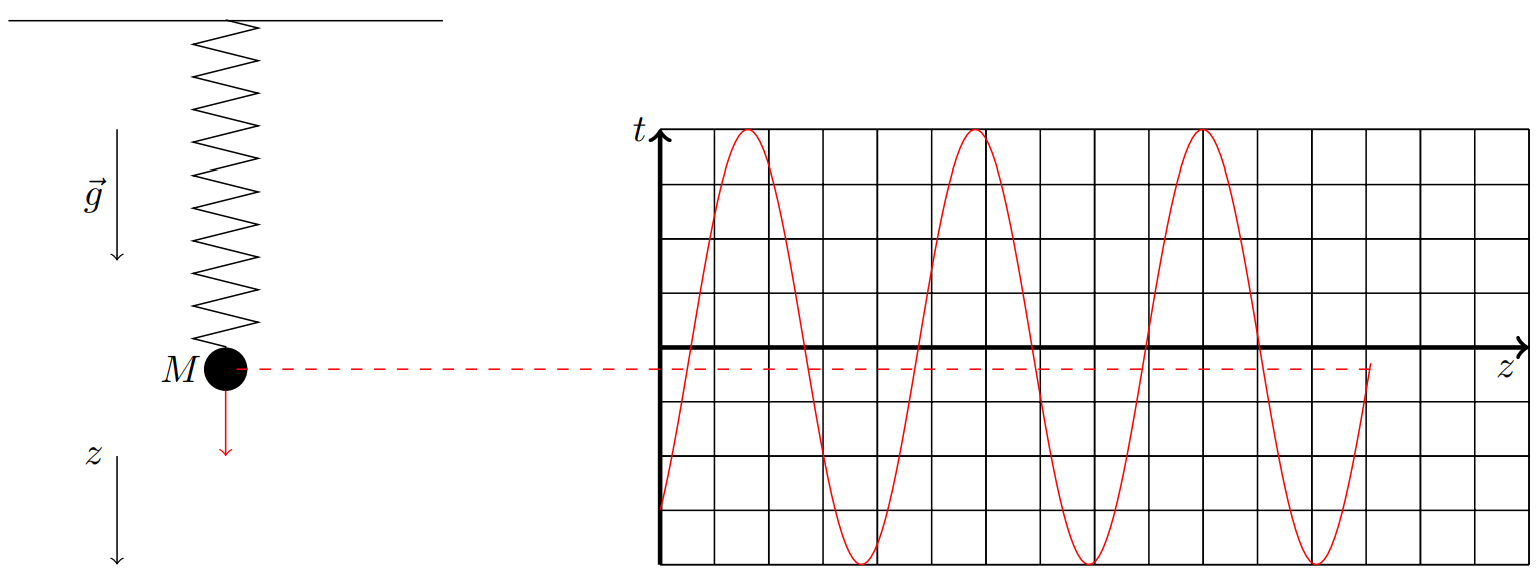
\includegraphics[scale = 0.5]{Images/ressort}
Equation différentielle : 
\begin{equation*}
\ddot x + \omega_0^2x =  0
\end{equation*}
\begin{itemize}
\item La fréquence : $f=\displaystyle\frac{\omega_{0}}{2\pi}$ (le nombre d'oscillations par seconde) 
\item La période : $T=\displaystyle\frac{2\pi}{\omega_{0}}=\displaystyle\frac{1}{f}$ ,  durée d'une oscillation
\end{itemize}
\end{frame}
\begin{frame}{Oscillateur harmonique III : Solutions du problème}

\begin{itemize}
    \item Equation horaire de l'oscillateur harmonique:  x(t)=A.\sin{(\omega t)}+B.\cos{(\omega t)} \newline
    OU \newline
    x(t)=C.\sin{(\omega t +\varphi)}
\end{itemize}

\begin{itemize}
    \item Equation de la vitesse de l'oscillateur harmonique : \newline
    $\dot{x}$(t)=$\omega$.A.\cos{(\omega t)}-$\omega$ B.\sin{(\omega t)}  \newline
    OU\newline
    \dot x(t)=$\omega$.C.\cos{(\omega t +\varphi)}
\end{itemize}

\begin{itemize}
    \item Equation de l'accélération de l'oscillateur harmonique :  $\ddot{x}$(t)=$-\omega^{2}$.A.\sin{(\omega t)}-$\omega^{2}$.B.\cos{(\omega t)} \newline
    OU\newline 
    \ddot x(t)=$-\omega^{2}$.C.\sin{(\omega t +\varphi)}
\end{itemize}
    
\end{frame}

\begin{frame}{Oscillateur harmonique IV : Point d'équilibre}
\begin{center}
    \definecolor{ffqqqq}{rgb}{1.,0.,0.}
\definecolor{qqffqq}{rgb}{0.,1.,0.}
\begin{tikzpicture}[line cap=round,line join=round,>=triangle 45,x=1.0cm,y=1.0cm]
\clip(1.57,-1.2) rectangle (11.,1.4);
\draw[line width=1.3pt, smooth,samples=100,domain=1.5707963267948966:10.995574287564276] plot[parametric] function{t,sin((t))};
\begin{scriptsize}
\draw [fill=qqffqq] (7.853981633974483,1.1) circle (3.5pt);
\draw [fill=ffqqqq] (4.71238898038469,-0.9) circle (3.5pt);
\end{scriptsize}
\end{tikzpicture}
\end{center}
\end{frame}


\begin{frame}{Le problème du pendule : Figure}
    \begin{figure}[h]
    \centering
    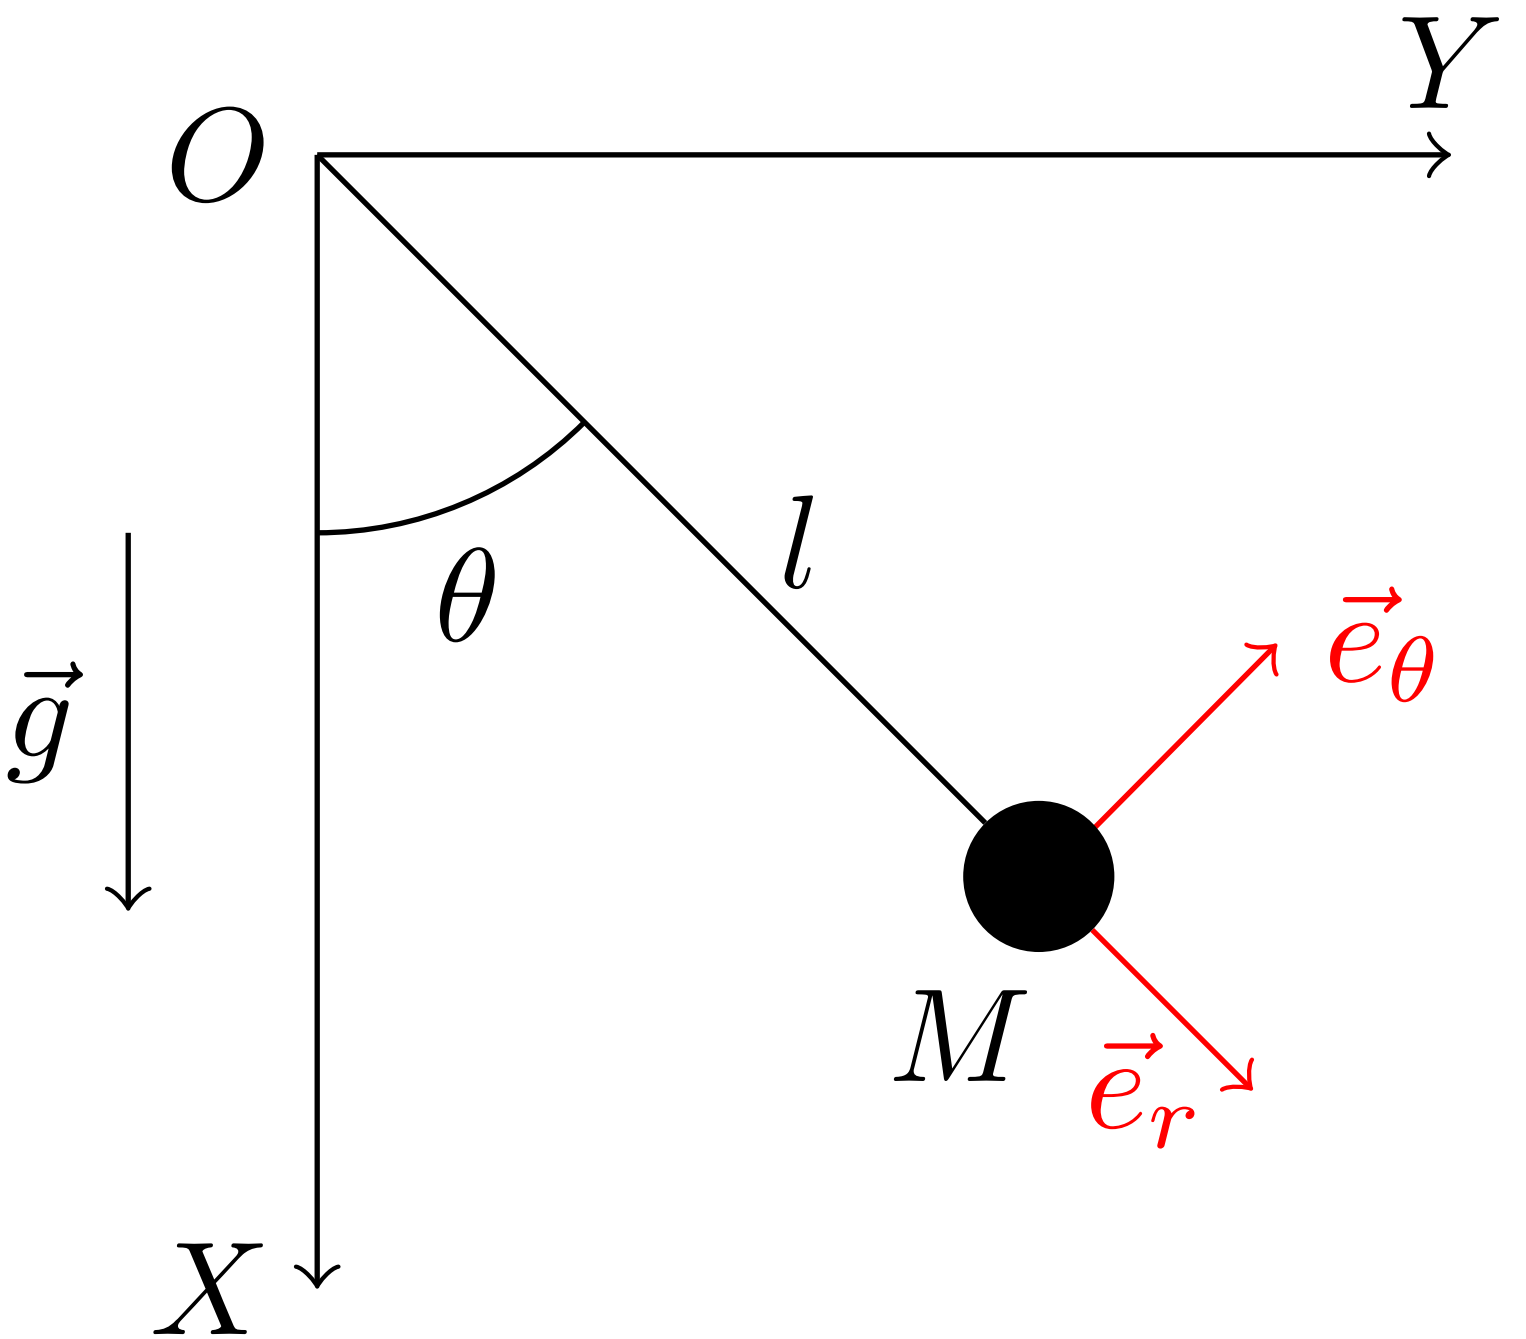
\includegraphics[scale = 0.4]{Images/Pendule}
    \caption{Représentation du problème en coordonnées polaires}
\end{figure}
\end{frame}
\begin{comment}

\begin{frame}{Coordonnées polaires: Partie I}
 \begin{figure}[h]
    \centering
    
\definecolor{qqqqcc}{rgb}{0.,0.,0.8}
\definecolor{wrwrwr}{rgb}{0.3803921568627451,0.3803921568627451,0.3803921568627451}
\definecolor{sexdts}{rgb}{0.1803921568627451,0.49019607843137253,0.19607843137254902}
\definecolor{rvwvcq}{rgb}{0.08235294117647059,0.396078431372549,0.7529411764705882}
\definecolor{dtsfsf}{rgb}{0.8274509803921568,0.1843137254901961,0.1843137254901961}
\begin{tikzpicture}[line cap=round,line join=round,>=triangle 45,x=9.23076923076923cm,y=9.23076923076923cm]
\begin{axis}[
x=9.23076923076923cm,y=9.23076923076923cm,
axis lines=middle,
ymajorgrids=false,
xmajorgrids=false,
xmin=-0.05,
xmax=0.6,
ymin=-0.05,
ymax=0.6,
xtick={-0.0},
ytick={-0.0},]
\clip(-0.05,-0.05) rectangle (0.6,0.6);
\draw [shift={(-0.05,-0.05)},line width=1.6pt,fill=black,fill opacity=0.10000000149011612] (0,0) -- (0.:0.14715816481548463) arc (0.:45.:0.14715816481548463) -- cycle;
\draw [line width=0.8pt,color=dtsfsf,domain=-0.05:0.6] plot(\x,{(-0.--0.35355339059327373*\x)/0.3535533905932738});
\draw [line width=0.4pt,color=rvwvcq,domain=-0.05:0.6] plot(\x,{(-0.35355339059327373-0.*\x)/-1.});
\draw [line width=0.4pt,color=sexdts] (0.3535533905932738,-0.05) -- (0.3535533905932738,0.6);
\draw [line width=0.4pt] (0.,0.) circle (3.263569759322527cm);
\draw [color=rvwvcq](0.002806511968452988,0.4145107916421979) node[anchor=north west] {$r\sin \theta$};
\draw [color=sexdts](0.35892927082192577,0.06427435938134453) node[anchor=north west] {$r\cos \theta$};
\draw [line width=0.4pt,dash pattern=on 2pt off 2pt,color=wrwrwr] (0.,0.) circle (4.615384615384615cm);
\draw [->,line width=0.8pt,color=wrwrwr] (0.3535533905932738,0.35355339059327373) -- (0.4242640687119286,0.42426406871192857);
\draw [->,line width=0.8pt,color=wrwrwr] (0.3535533905932738,0.35355339059327373) -- (0.280617318100129,0.4264894630864185);
\draw [color=rvwvcq](0.2794638618215641,0.4645445676794626) node[anchor=north west] {$\mathbf{e}_\theta$};
\draw [color=rvwvcq](0.3765882505997839,0.4792603841610111) node[anchor=north west] {$\mathbf{e}_r$};
\draw [color=rvwvcq](0.002806511968452988,0.4145107916421979) node[anchor=north west] {$r\sin \theta$};
\draw (0.14260676854316337,0.11136497212229961) node[anchor=north west] {$\theta$};
\draw (0.14260676854316337,0.11136497212229961) node[anchor=north west] {$\theta$};
\draw (0.5311043236560428,0.05397328784426061) node[anchor=north west] {$x$};
\draw (0.005749675264762681,0.5793279362355407) node[anchor=north west] {$y$};
\begin{scriptsize}
\draw [fill=qqqqcc] (0.,0.) circle (2.0pt);
\draw[color=qqqqcc] (0.020465491746311144,0.0664817318535768) node {$O$};
\end{scriptsize}
\end{axis}
\end{tikzpicture}
    \caption{Axes et points en coordonnées polaires}
    \label{fig:polar}
\end{figure}

\end{frame}
\begin{frame}{Coordonnées polaires: Partie II}
    Les relations liant les coordonnées cartésiennes aux coordonnées polaires sont les suivantes :
\begin{equation}    
\begin{cases} x = r\cos{\theta} \\
y = r\sin{\theta} 
\end{cases}
\end{equation}

\begin{itemize}

   \item Vitesse en coordonnées polaires :  $\vec{v}= \dot{r}\mathbf{e}_r+r\dot \theta\mathbf{e}_\theta $
 \end{itemize}  
 \begin{itemize}
   \item  Accélération en coordonnées polaires : \newline
   $\vec{a} = (\ddot{r}$- r $\dot \theta^{2})\mathbf{e}_r + (2\dot r \dot \theta + r\ddot \theta) \mathbf{e}_\theta$ \\
\end{itemize}
\end{frame}
\begin{frame}{Oscillateur harmonique: Partie I}
Force de rappel (Loi de Hooke) :  \[ \vec{F_e} = -k \vec{d} = -k(x - x_0) \vec{e_x} \]    \newline
Equation différentielle : 
\begin{equation*}
    \ddot x + \omega_0^2x =  0
\end{equation*}
avec $\omega_{0}$ la pulsation propre de l'oscillateur. De cette dernière on définira deux nouvelles grandeurs: \newline
\begin{itemize}
\item La fréquence : $f=\displaystyle\frac{\omega_{0}}{2\pi}$ (le nombre d'oscillations par seconde) 
\item La période : $T=\displaystyle\frac{2\pi}{\omega_{0}}=\displaystyle\frac{1}{f}$ , représentant la durée d'une oscillation
\end{itemize}



\end{frame}
\begin{frame}{Oscillateur harmonique : Partie II}
    Par ailleurs, la pulsation de l'oscillateur ne dépend que de deux paramètres : $k$ la constante de raideur du ressort et $m$ la masse de la bille. La relation les liant est donnée par :
\begin{itemize}
    \item $\omega_{0}=\displaystyle\sqrt{\frac{k}{m}}$
\end{itemize}
Limites du modèle : \newline
- moins précis pour des oscillations de plus grande amplitude.\newline
-Dans le monde réel il n'y a pas de une conservation totale de l'énergie (notamment en raison des frottements)\newline
\end{frame}
\begin{frame}{Oscillateur harmonique : Solutions du problème}

\begin{itemize}
    \item Equation horaire de l'oscillateur harmonique:  x(t)=A.\sin{(\omega t)}+B.\cos{(\omega t)} \newline
    OU \newline
    x(t)=C.\sin{(\omega t +\varphi)}
\end{itemize}



\begin{itemize}
    \item Equation de la vitesse de l'oscillateur harmonique : \newline
    $\dot{x}$(t)=$\omega$.A.\cos{(\omega t)}-$\omega$ B.\sin{(\omega t)}  \newline
    OU\newline
    x(t)=$\omega$.C.\cos{(\omega t +\varphi)}
\end{itemize}

\begin{itemize}
    \item Equation de l'accélération de l'oscillateur harmonique :  $\ddot{x}$(t)=$-\omega^{2}$.A.\sin{(\omega t)}-$\omega^{2}$.B.\cos{(\omega t)} \newline
    OU\newline 
    x(t)=$-\omega^{2}$.C.\sin{(\omega t +\varphi)}
\end{itemize}
    
\end{frame}
\begin{frame}{Le problème du pendule}
Enoncé : On considère un pendule constitué d'un poids M de masse $m$, suspendu au bout d'un fil de longueur $l$ à un angle initial $\theta_0$ et à une vitesse initiale nulle. On place l'origine $O$ au point d'accroche du fil et on définit $\theta$, l'angle entre l'axe $Ox$ et le fil. Le but de l'exercice est de déterminer l'équation horaire de la masse en négligeant toutes sortes de frottements et en supposant des oscillations de faibles amplitudes autour de l'axe $Ox$.\\
    
\end{frame}
\begin{frame}{Le problème du pendule : Figure}
    \begin{figure}[h]
    \centering
    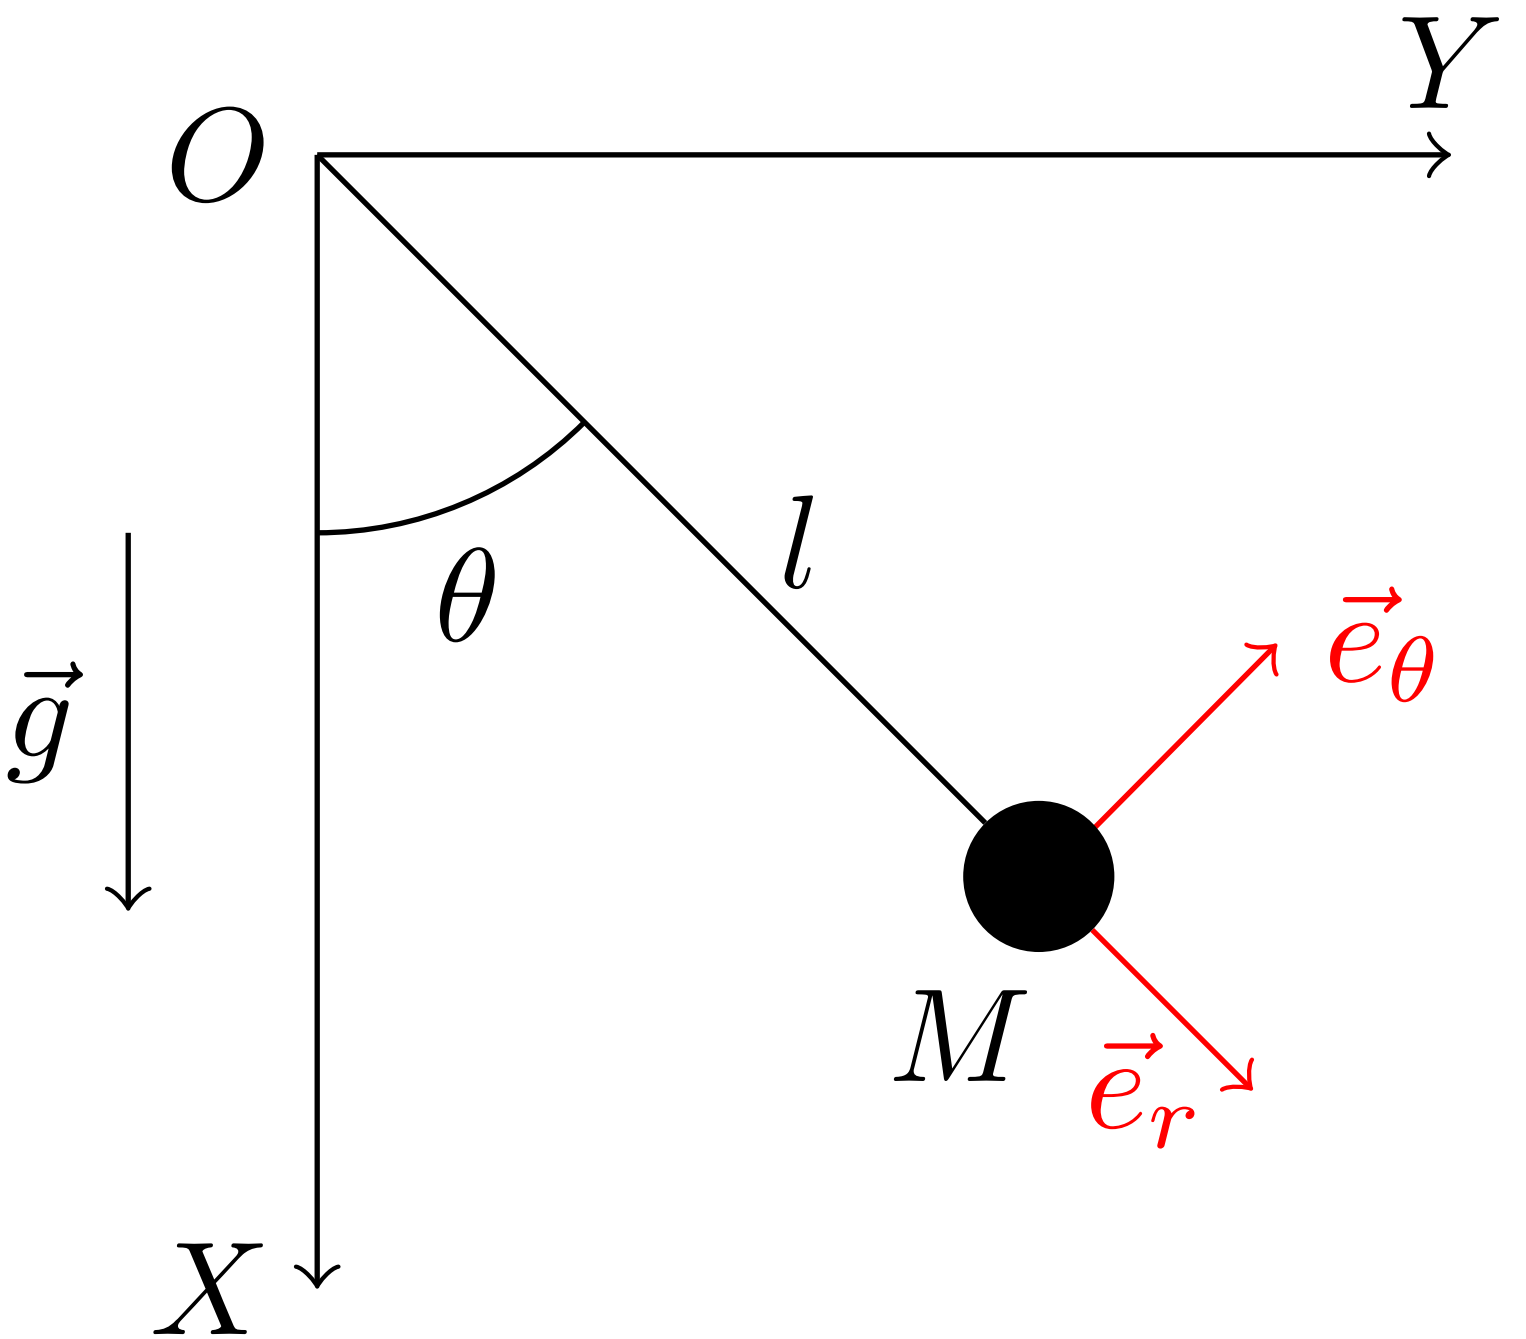
\includegraphics[scale = 0.4]{Images/Pendule}
    \caption{Représentation du problème en coordonnées polaires}
\end{figure}
\end{frame}
\begin{frame}{Le problème du pendule: Principales étapes de résolution}
\begin{enumerate}
    \item Choisir le bon système de coordonnées
    \item Faire le bilan des forces, utiliser la seconde loi de Newton
    \item A l'aide des données obtenues, résoudre les équations du mouvement
\end{enumerate}

Remarque: De manière générale, les $3$ grandes étapes montrées ci-dessus seront celles à suivre pour tout problème de mécanique.
    
\end{frame}
\end{comment}
\end{document}
